% NetMob 2026 poster, A0 portrait (841 x 1189 mm). pdfLaTeX.
\documentclass{article}
\usepackage[paperwidth=841mm,paperheight=1189mm,margin=0mm]{geometry}
\usepackage[T1]{fontenc}
\usepackage{lmodern}
\usepackage{tgheros}
\renewcommand{\familydefault}{\sfdefault}
\usepackage{xcolor}
\usepackage{tikz}
\usetikzlibrary{positioning,calc,fit,decorations.pathreplacing}
\usepackage{pgfplots}
\pgfplotsset{compat=1.17}
\usepackage{booktabs}
\usepackage{tabularx}
\usepackage{enumitem}
\usepackage{qrcode}
\pagestyle{empty}
\setlength{\parindent}{0pt}
\setlength{\parskip}{5mm}

\definecolor{navy}{HTML}{14213D}
\definecolor{accent}{HTML}{C8102E}
\definecolor{ink}{HTML}{1F2937}
\definecolor{muted}{HTML}{5B6472}
\definecolor{scr}{HTML}{DCE6F5}
\definecolor{rel}{HTML}{DCEFE3}
\definecolor{hdr}{HTML}{EEF0F3}

\newcommand{\body}{\fontsize{29}{38}\selectfont}
\renewcommand{\small}{\fontsize{24}{31}\selectfont}
\newcommand{\sect}[1]{\par\vfill\vspace{8mm}%
  {\color{navy}\fontsize{46}{52}\selectfont\bfseries #1\par}%
  \vspace{2mm}{\color{accent}\rule{\linewidth}{1.2mm}}\par\vspace{2mm}}
\newcommand{\firstsect}[1]{%
  {\color{navy}\fontsize{46}{52}\selectfont\bfseries #1\par}%
  \vspace{2mm}{\color{accent}\rule{\linewidth}{1.2mm}}\par\vspace{2mm}}
\newcommand{\fig}[1]{\par\vspace{1mm}{\small\color{muted}#1\par}}
\setlist{nosep, leftmargin=9mm, itemsep=2mm, label=\textbullet}
\setlength{\tabcolsep}{4mm}
\renewcommand{\arraystretch}{1.25}

\pgfplotsset{every axis/.append style={
  font=\small, width=0.93\linewidth, height=95mm, scale only axis=false,
  grid=major, grid style={gray!25}, axis line style={muted},
  tick style={muted}, label style={font=\small}, tick label style={font=\small},
  legend style={font=\small, draw=none, fill=white, fill opacity=0.85, text opacity=1}}}

\begin{document}
\color{ink}
\begin{tikzpicture}[remember picture, overlay]
  \fill[navy] (current page.north west) rectangle ([yshift=-165mm]current page.north east);
  \fill[accent] ([yshift=-165mm]current page.north west) rectangle ([yshift=-168mm]current page.north east);
\end{tikzpicture}

% ---------------------------------------------------------------- header
\vspace*{24mm}
\hspace*{32mm}\begin{minipage}[t]{640mm}
  {\color{white}\fontsize{78}{86}\selectfont\bfseries BUBBLE-BLUE: private group messaging\\[2mm]
   over an open Bluetooth LE mesh\par}
  \vspace{9mm}
  {\color{white}\fontsize{32}{40}\selectfont Paul-Maxence Baraton$^1$, Nadjib Achir$^1$,
   Philippe Jacquet$^1$, Wilfred Doré$^2$\par}
  \vspace{3mm}
  {\color{white!80!navy}\fontsize{25}{32}\selectfont $^1$Inria, France \qquad $^2$Qualcomm, France
   \qquad paul-maxence.baraton@inria.fr\par}
\end{minipage}\hfill
\begin{minipage}[t]{110mm}
  \vspace{-2mm}\centering
  \colorbox{white}{\qrcode[height=78mm]{https://arxiv.org/abs/2509.00967}}\\[2mm]
  {\color{white!80!navy}\fontsize{19}{23}\selectfont arXiv:2509.00967}
\end{minipage}\hspace*{32mm}

\vspace{46mm}
\body
\hspace*{30mm}%
% ================================================================ column 1
\begin{minipage}[t][935mm][t]{245mm}
\firstsect{1\enspace Problem and contribution}
Where infrastructure is absent, saturated or not trusted (a crowd, a
disaster site, an event), devices can still reach each other over
Bluetooth. Existing Bluetooth meshes either require provisioning, so a
stranger cannot relay, or let every relay read every message [2--4].

BUBBLE-BLUE separates two things:
\begin{itemize}
  \item the \textbf{topological mesh} is open: any node may join and
        relay, including traffic it cannot decrypt;
  \item a \textbf{bubble} is a group defined by a key: only its members
        read its messages.
\end{itemize}
We contribute the BLE transport (L2CAP connection-oriented channels, no
pairing), the frame format, a revocation protocol, and measurements on
six boards, in a room and across a building.

\vspace{4mm}
{\small
\begin{tabularx}{\linewidth}{@{}Xlll@{}}
\toprule
System & Backbone & Open relay & Group privacy \\
\midrule
SIG Mesh [2] & provisioned & no & network key \\
BitChat [3] & none & n/a & per channel \\
Briar [5] & contacts & no & end-to-end \\
Reticulum [6] & identities & no & end-to-end \\
\textbf{BUBBLE-BLUE} & \textbf{elected CDS} & \textbf{yes} & \textbf{group key} \\
\bottomrule
\end{tabularx}}
\fig{Table 1. Where BUBBLE-BLUE sits. ``Open relay'': a node forwards a
frame it cannot decrypt.}

\sect{2\enspace Design}
\begin{center}
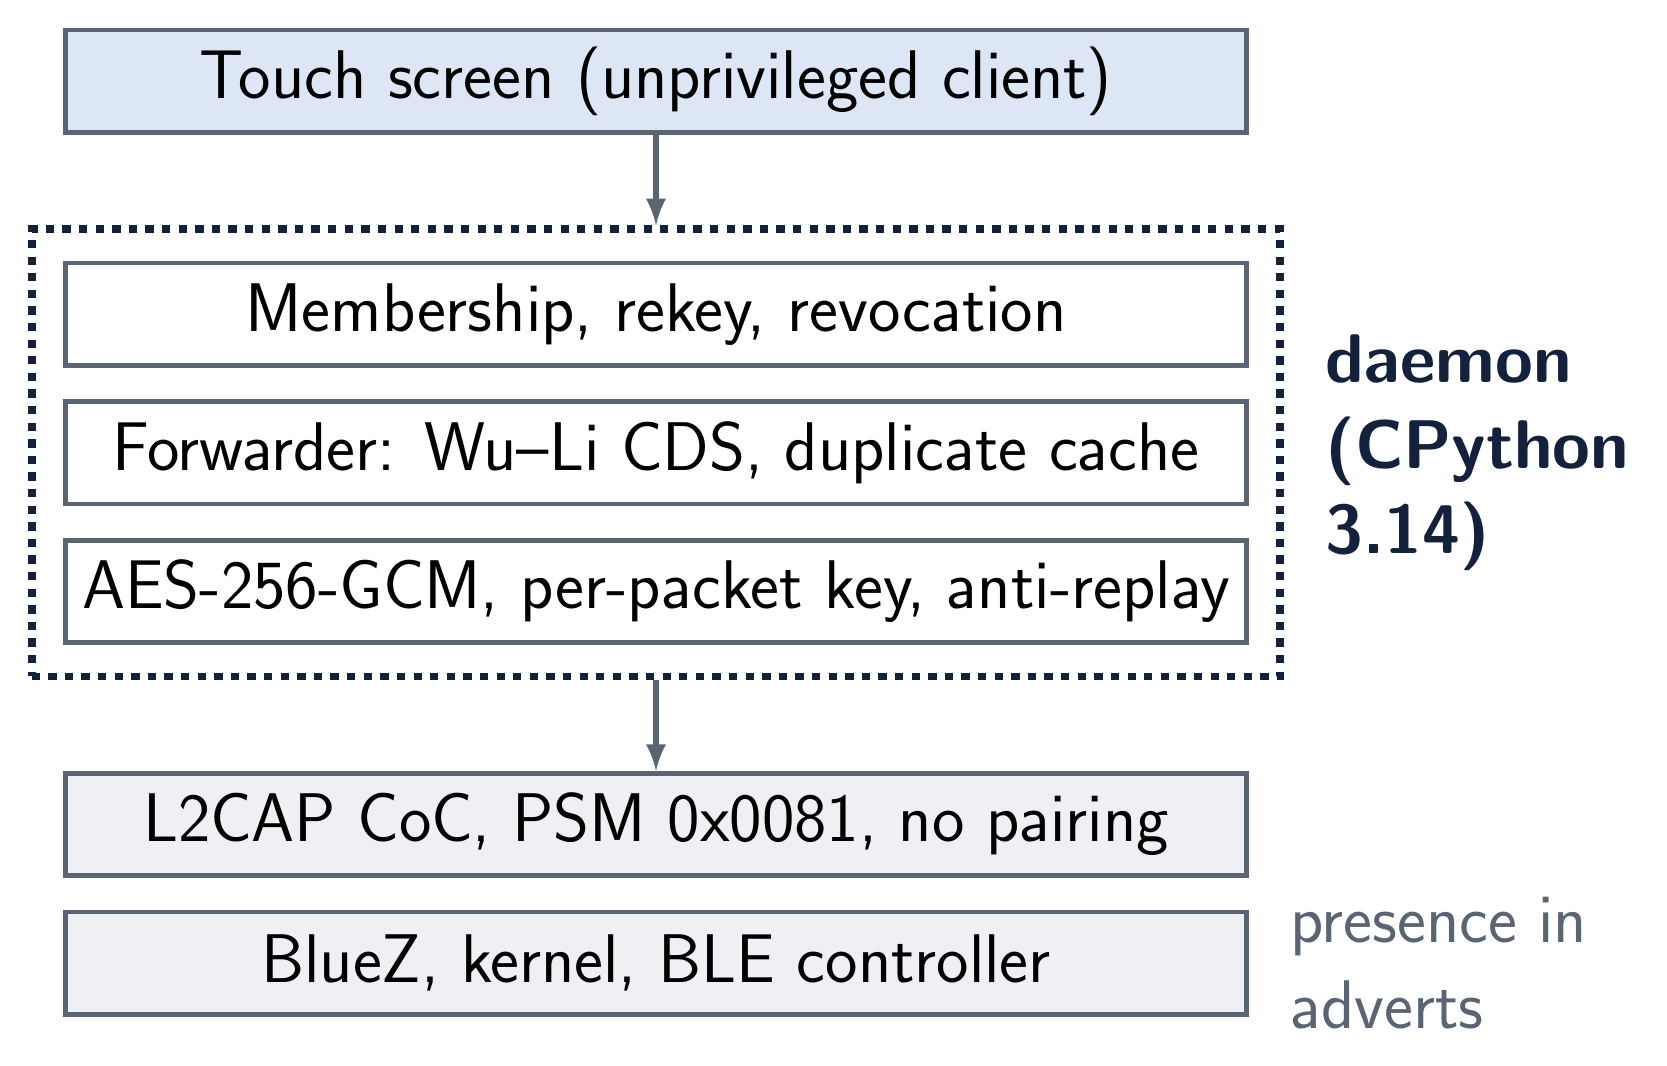
\begin{tikzpicture}[font=\small, node distance=4mm,
  b/.style={draw=muted, fill=#1, minimum width=150mm, minimum height=13mm, align=center, line width=0.6mm},
  b/.default=white]
  \node[b=scr] (ui) {Touch screen (unprivileged client)};
  \node[b, below=16mm of ui] (mem) {Membership, rekey, revocation};
  \node[b, below=of mem] (fwd) {Forwarder: Wu--Li CDS, duplicate cache};
  \node[b, below=of fwd] (sec) {AES-256-GCM, per-packet key, anti-replay};
  \node[b=hdr, below=16mm of sec] (l2) {L2CAP CoC, PSM 0x0081, no pairing};
  \node[b=hdr, below=of l2] (bz) {BlueZ, kernel, BLE controller};
  \node[draw=navy, line width=1mm, dashed, inner sep=4mm, fit=(mem)(sec)] (d) {};
  \node[anchor=west, text=navy, font=\small\bfseries, align=left] at ([xshift=4mm]d.east) {daemon\\(CPython\\3.14)};
  \draw[-latex, line width=0.8mm, muted] (ui) -- (d.north -| ui);
  \draw[-latex, line width=0.8mm, muted] (d.south -| l2) -- (l2);
  \node[anchor=west, text=muted, font=\small, align=left] at ([xshift=4mm]bz.east) {presence in\\adverts};
\end{tikzpicture}
\end{center}
\fig{Figure 1. One daemon per board owns the radio; screens are clients.}

\begin{center}
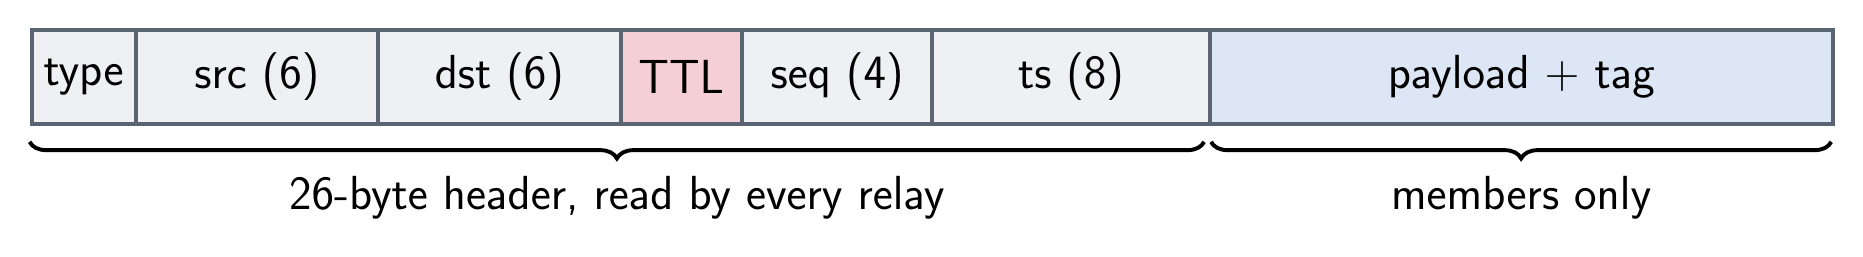
\begin{tikzpicture}[font=\fontsize{19}{23}\selectfont, x=2.2mm, y=1mm,
  f/.style={draw=muted, line width=0.5mm, minimum height=12mm, inner sep=0pt, anchor=south west}]
  \foreach \x/\w/\t/\c in {0/6/type/hdr, 6/14/src (6)/hdr, 20/14/dst (6)/hdr,
                           34/7/TTL/accent!20, 41/11/seq (4)/hdr, 52/16/ts (8)/hdr}
    \node[f, fill=\c, minimum width=\w*2.2mm] at (\x,0) {\t};
  \node[f, fill=scr, minimum width=36*2.2mm] at (68,0) {payload + tag};
  \draw[decorate, decoration={brace, amplitude=6pt, mirror}, line width=0.5mm] (0,-2) -- (67.8,-2)
    node[midway, below=3mm] {26-byte header, read by every relay};
  \draw[decorate, decoration={brace, amplitude=6pt, mirror}, line width=0.5mm] (68.2,-2) -- (104,-2)
    node[midway, below=3mm] {members only};
\end{tikzpicture}
\end{center}
\fig{Figure 2. Frame format. The header is authenticated as associated data,
except TTL, which relays decrement.}

\begin{itemize}
  \item \textbf{Links.} A node advertises an anonymous identifier, a relay
        flag and its L2CAP address (Company ID 0xFFFF, the SIG test
        value). Neighbours open a CoC at security level \emph{low}.
  \item \textbf{Keys.} $K_{\mathrm{pkt}} = \mathrm{HKDF}_{\mathrm{SHA256}}(K;\,
        \mathit{src}\,\|\,\mathit{seq}\,\|\,\mathit{ts})$, so a zero GCM
        nonce is never reused under one key.
  \item \textbf{Relays.} Each node applies the Wu--Li rule [7] to its
        two-hop view; marked nodes form a connected dominating set and
        are the only ones to rebroadcast.
  \item \textbf{Revocation.} The coordinator (smallest anonymous
        identifier) floods a new group key wrapped under pairwise X25519
        keys, skipping the excluded member. That member keeps relaying.
\end{itemize}
\end{minipage}%
\hspace{20mm}%
% ================================================================ column 2
\begin{minipage}[t][935mm][t]{245mm}
\firstsect{3\enspace Threat model}
{\small
\begin{tabularx}{\linewidth}{@{}>{\raggedright\arraybackslash}p{58mm}>{\raggedright\arraybackslash}X@{}}
\toprule
Adversary & What it obtains \\
\midrule
Passive radio & who transmits, to which address, how far a frame may still go, and timing. Not the text. \\
Non-member relay & can drop or delay frames and rewrite TTL. Cannot read or forge a message. \\
Active outsider & can flood junk or pre-empt a (source, sequence) pair in relay caches: selective loss. \\
Member & controlling its address, can grind its identifier to become coordinator. \\
Revoked member & keeps relaying; cannot read after the rekey. \\
\bottomrule
\end{tabularx}}
\fig{Table 2. Limits we accept in this prototype. The Bluetooth address is
stable, so a bond-free mesh does not give location privacy.}

Revocation is safe only after the newcomer's public key has been
announced (ANNOUNCE every 30\,s). Before that, the coordinator refuses
it: this defines a join window.

\sect{4\enspace Testbed}
{\small
\begin{tabularx}{\linewidth}{@{}l>{\raggedright\arraybackslash}X>{\raggedright\arraybackslash}X@{}}
\toprule
 & Thundercomm RUBIK Pi 3 & Arduino UNO Q \\
\midrule
Role & screen & relay \\
SoC & Qualcomm QCS6490 & Qualcomm QRB2210 \\
OS, kernel & Ubuntu 24.04, 6.8 & Debian 13, 7.0 \\
BlueZ & 5.72 & 5.82 \\
Controller & BCM4345C5 (BT 5.0) & WCN399x (BT 5.1) \\
\bottomrule
\end{tabularx}}
\fig{Table 3. Three of each board. The daemon needs CPython 3.14 for the LE
address family of \texttt{socket}.}

\begin{center}
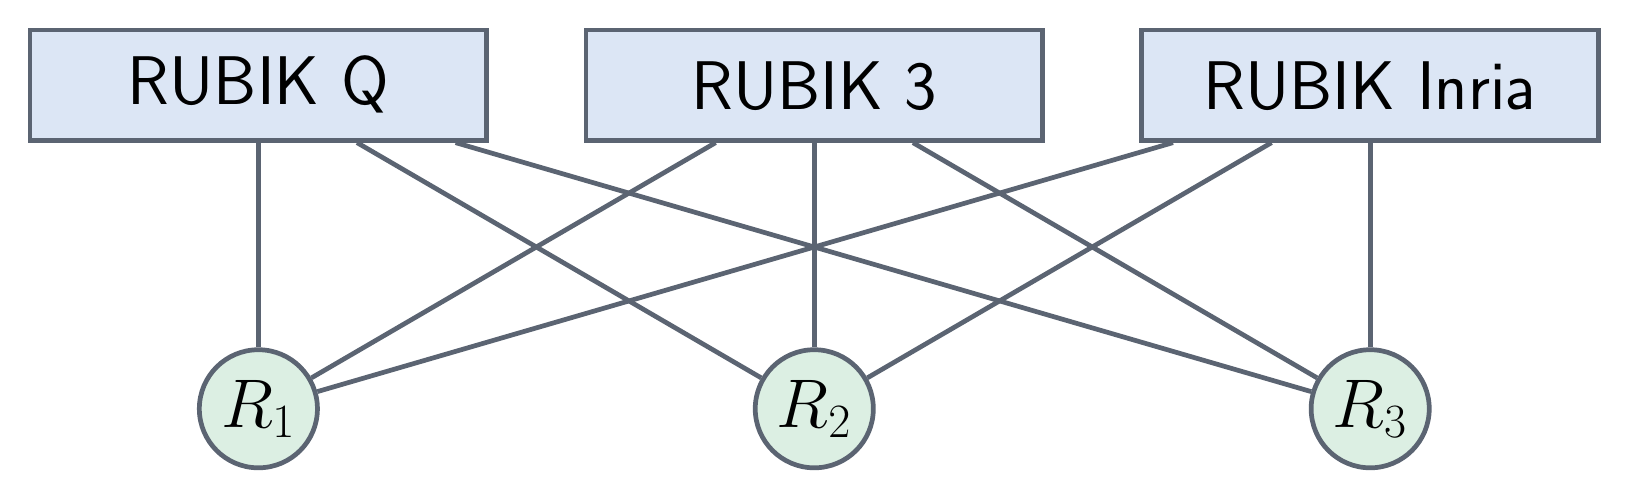
\begin{tikzpicture}[font=\small,
  s/.style={draw=muted, line width=0.6mm, fill=scr, minimum width=58mm, minimum height=14mm},
  r/.style={draw=muted, line width=0.6mm, circle, fill=rel, minimum size=15mm, inner sep=0pt}]
  \node[s] (a) {RUBIK Q};
  \node[s, right=12mm of a] (b) {RUBIK 3};
  \node[s, right=12mm of b] (c) {RUBIK Inria};
  \node[r, below=26mm of a] (r1) {$R_1$};
  \node[r, below=26mm of b] (r2) {$R_2$};
  \node[r, below=26mm of c] (r3) {$R_3$};
  \foreach \x in {a,b,c} \foreach \y in {r1,r2,r3} \draw[muted, line width=0.6mm] (\x)--(\y);
\end{tikzpicture}
\end{center}
\fig{Figure 3. The stand: on a table the link graph is $K_{3,3}$, so every
message between screens crosses a relay that is not in the group.}

UNO Q relays always dial; their kernel leaks L2CAP signalling
identifiers (fixed upstream, 6e1930ece855), so links are recycled, and a
watchdog reloads a controller that stops answering.

\sect{5\enspace Results on the stand}
{\small
\begin{tabularx}{\linewidth}{@{}Xr@{}}
\toprule
Messages received by the five other boards & 75/75 \\
Six-node manual soak & 427/429 \\
Rebooted screen reads the group, after daemon start & 4.4\,s \\
Relay with a cut controller reads again, no reboot & 130\,s \\
Departure detected (3 missed Hellos, 15\,s) & 17--21\,s \\
Revoked board reads the next message (2 trials) & no \\
AES-GCM, 470 B, RUBIK / UNO Q (pkt/s) & 173k / 30k \\
Sustained load, RUBIK / UNO Q (msg/s) & 30 / 10 \\
\bottomrule
\end{tabularx}}
\fig{Table 4. The two losses of the soak are the first message (before
convergence) and the last (during shutdown). Above 10\,msg/s the UNO Q
runs out of L2CAP identifiers: the bottleneck is its Bluetooth stack,
not the cryptography.}

\sect{6\enspace Simulation: TTL as hop budget}
The shipped forwarder on random geometric graphs (nominal degree 6,
measured degree below), probed from three sources per draw.

{\small
\begin{tabularx}{\linewidth}{@{}XXXXX@{}}
\toprule
nodes & degree & ecc.\ (hops) & min TTL & TTL\,10 \\
\midrule
10 & 3.9 & 4 & 4 & 100\,\% \\
20 & 4.3 & 8 & 8 & 100\,\% \\
30 & 3.3 & 11 & 11 & 93\,\% \\
50 & 5.2 & 13 & 13 & 94\,\% \\
100 & 5.2 & 19 & 19 & 23\,\% \\
\bottomrule
\end{tabularx}}
\fig{Table 5. The minimum TTL that reaches every node equals the worst
source's eccentricity on every draw. Revocation (n = 6 to 30): no
stranded member, no leak to the excluded one; its cost grows roughly
linearly per node.}
\end{minipage}%
\hspace{20mm}%
% ================================================================ column 3
\begin{minipage}[t][935mm][t]{245mm}
\firstsect{7\enspace Four hops across a building}
With the boards about 15\,m apart and one relay off, the mesh formed a
line by itself. On-board logs, clocks within 50\,ms; 79 messages.

\vspace{6mm}


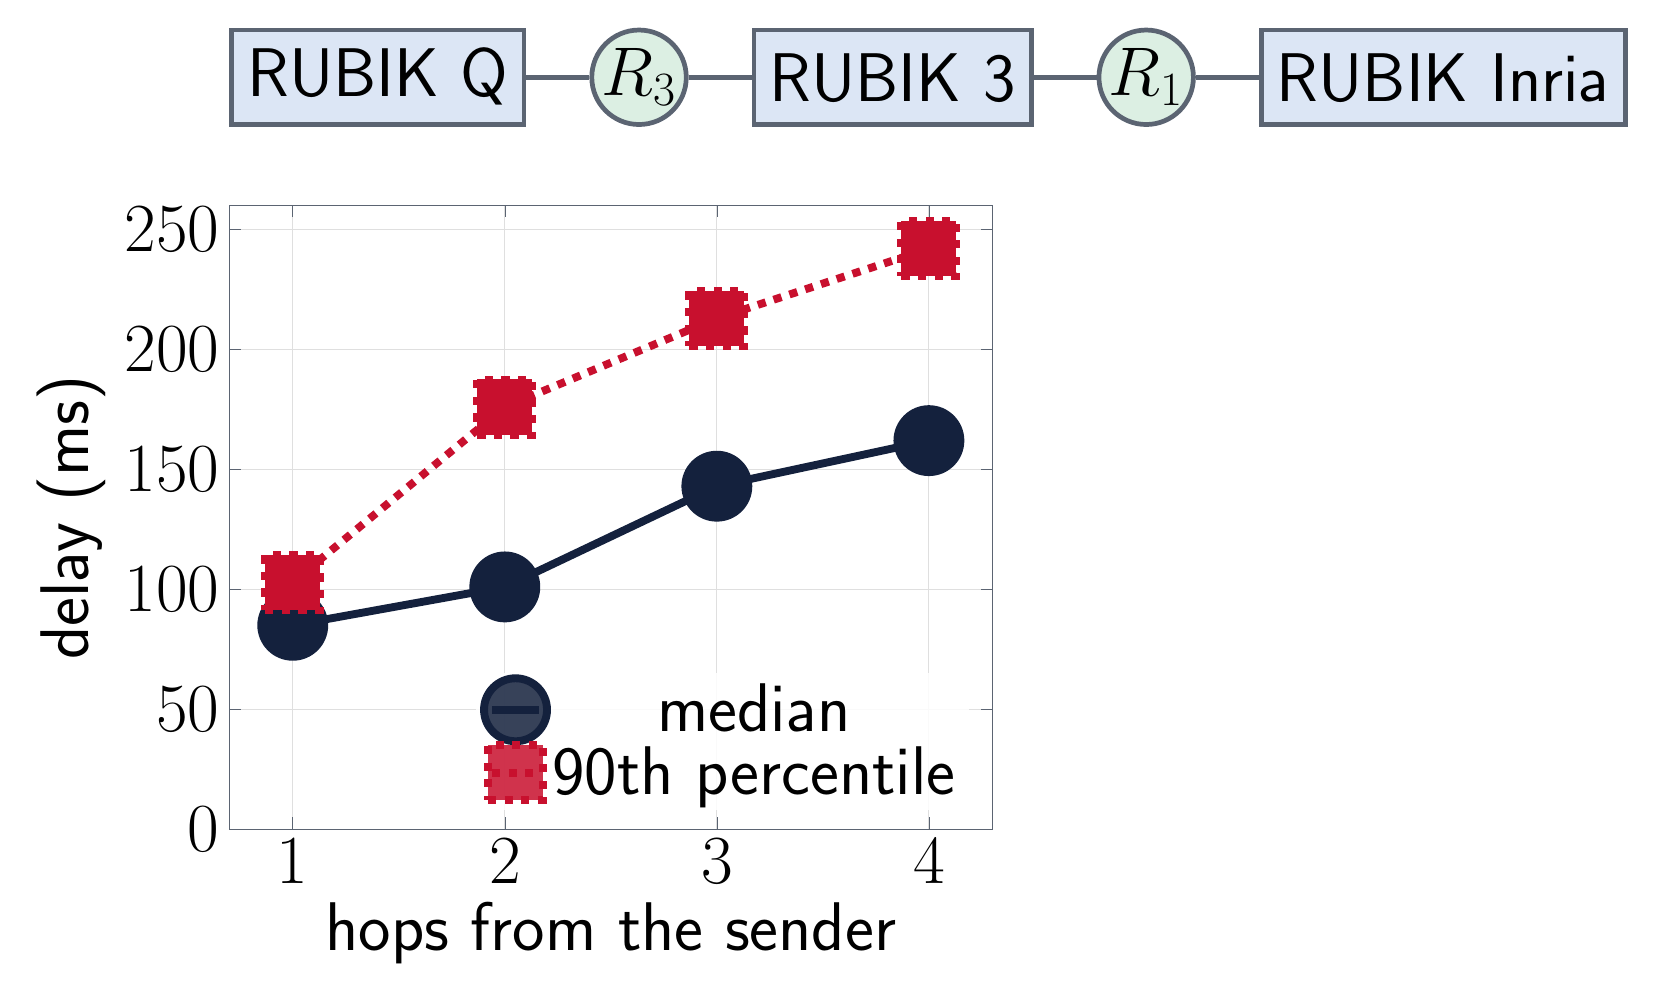
\begin{tikzpicture}[
  s/.style={draw=muted, line width=0.6mm, fill=scr, minimum height=12mm, inner sep=2mm, font=\small},
  r/.style={draw=muted, line width=0.6mm, circle, fill=rel, minimum size=12mm, inner sep=0pt, font=\small}]
\begin{axis}[height=95mm, xlabel={hops from the sender}, ylabel={delay (ms)},
  xmin=0.7, xmax=4.3, ymin=0, ymax=260, xtick={1,2,3,4}, legend pos=south east]
\addplot[line width=1mm, mark=*, mark size=4mm, navy] coordinates {(1,85) (2,101) (3,143) (4,162)};
\addlegendentry{median}
\addplot[line width=1mm, dashed, mark=square*, mark size=3.5mm, accent] coordinates {(1,103) (2,176) (3,213) (4,242)};
\addlegendentry{90th percentile}
\end{axis}
\node[s, anchor=south west] (a) at ([yshift=10mm]current axis.north west) {RUBIK Q};
\node[r, right=8mm of a] (b) {$R_3$};
\node[s, right=8mm of b] (c) {RUBIK 3};
\node[r, right=8mm of c] (d) {$R_1$};
\node[s, right=8mm of d] (e) {RUBIK Inria};
\foreach \u/\v in {a/b,b/c,c/d,d/e} \draw[line width=0.6mm, muted] (\u)--(\v);
\end{tikzpicture}
\fig{Figure 4. Send-to-display delay. The far end received 76/79, missing
the three sent while the line formed. Carried away, its link held to
about 30\,m. With the sender's only relay unplugged, the line was dark
for 95\,s: a line has no detour.}

\sect{8\enspace 8.2 hours on battery}
The stand on battery, one message every 30\,s from RUBIK Q: 988
messages, 4\,915 expected receptions.

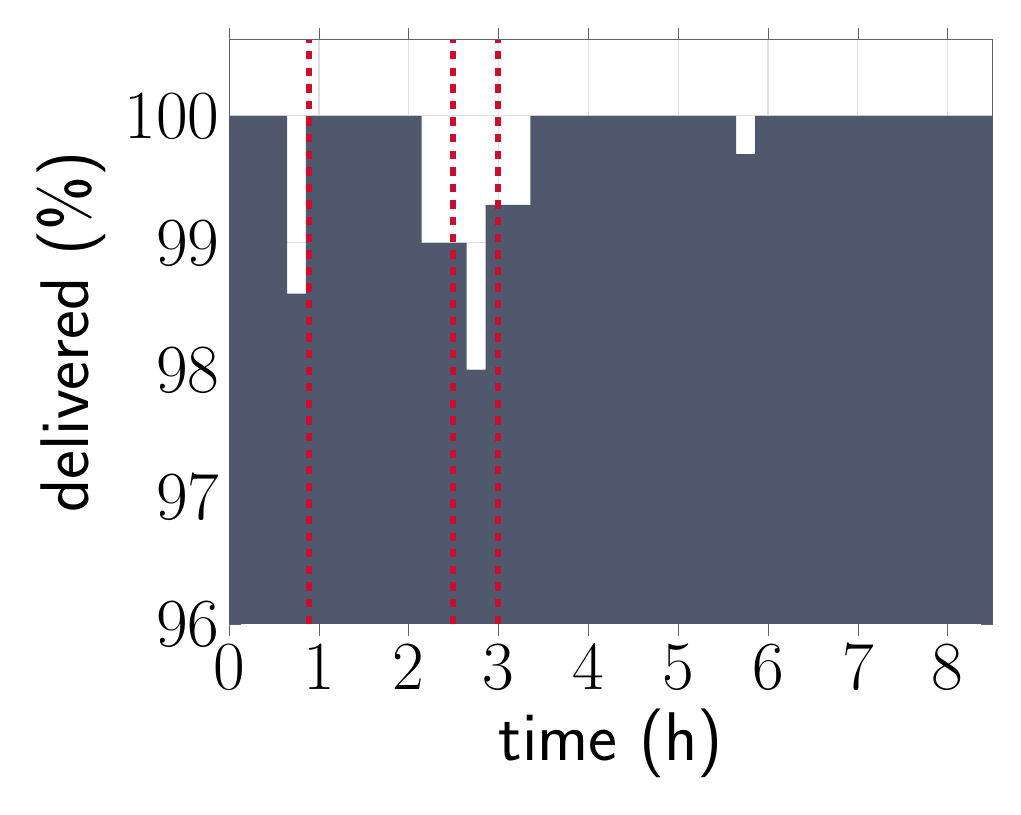
\begin{tikzpicture}
\begin{axis}[height=90mm, xlabel={time (h)}, ylabel={delivered (\%)},
  xmin=0, xmax=8.5, ymin=96, ymax=100.6, xtick={0,1,...,8}, ytick={96,97,98,99,100},
  ybar, bar width=9mm, bar shift=0pt]
\addplot[fill=navy!75, draw=none] coordinates {(0.25,100) (0.75,98.6) (1.25,100) (1.75,100)
  (2.25,99.0) (2.75,98.0) (3.25,99.3) (3.75,100) (4.25,100) (4.75,100) (5.25,100) (5.75,99.7)
  (6.25,100) (6.75,100) (7.25,100) (7.75,100) (8.12,100)};
\draw[accent, line width=0.8mm, dashed] (axis cs:0.89,96) -- (axis cs:0.89,100.6);
\draw[accent, line width=0.8mm, dashed] (axis cs:2.49,96) -- (axis cs:2.49,100.6);
\draw[accent, line width=0.8mm, dashed] (axis cs:2.99,96) -- (axis cs:2.99,100.6);
\end{axis}
\end{tikzpicture}
\fig{Figure 5. Delivery per 30-minute bin. Dashed: controller reloads on two
UNO Q relays (four reloads, about two minutes deaf each).}

{\small
\begin{tabularx}{\linewidth}{@{}Xr@{}}
\toprule
Received by the screens / by the relays & 100\,\% / 99.3\,\% \\
Delay, median / 90th / 99th percentile & 80 / 118 / 188\,ms \\
Boards still up when stopped & 6/6 \\
\bottomrule
\end{tabularx}}

\sect{9\enspace Defects found by measuring}
\begin{enumerate}[label=\arabic*., leftmargin=10mm]
  \item ANNOUNCE and data shared one anti-replay window: a data frame
        with an ANNOUNCE's sequence was dropped everywhere. \emph{Fixed,
        regression test.}
  \item On a sparse 30-node graph, four nodes elected themselves
        coordinator. \emph{Fixed: one membership view, regression test.}
  \item A restarted sender starts its sequence numbers again from zero,
        and every receiver's window silently drops it. \emph{Open:
        sequence numbers must survive a restart.}
\end{enumerate}

\sect{10\enspace Limits and next steps}
The default TTL\,10 spans about twenty nodes at this density; a
single relay is a single point of failure on a line. Next: an Android port of the CoC transport, energy of
the crypto path versus the radio, and replaying the protocol on the
contact graph that the link logs already record, to see how election and
revocation behave when people move.

\vspace{6mm}
{\fontsize{16}{20}\selectfont\color{muted}
[1] N. Achir, P. Jacquet, BUBBLE-BLUE, arXiv:2509.00967, 2025.
[2] Bluetooth SIG, Mesh Profile 1.0, 2017.
[3] J. Dorsey et al., BitChat, 2025.
[4] M. R. Albrecht et al., Breaking Bridgefy, CT-RSA 2021.
[5] Briar Project.
[6] M. Qvist, Reticulum.
[7] J. Wu, H. Li, connected dominating sets, DIAL-M 1999.
\par\vspace{3mm}
Boards provided by the Qualcomm University Platforms program.\par}
\end{minipage}
\end{document}
